\chapter{Introduction}
\chaptermark{Introduction}

\textit{Parts of this introduction have been published as a review article in BMC Biology. Sections marked with an ($ ^*$) have been reproduced, with minor modifications to the text. The published article is reproduced in full in the Appendices. 
}

In this introduction, I will start by briefly describing the main population genetic processes that will be discussed in this thesis. I will then describe how population genetic models can be used to make inferences from genomic data. I will end by describing the state of research in population genomics, with particular regard to natural selection, and describe the main aims of this thesis.

\section[Core concepts]{Core concepts in evolutionary genetics}

Evolution is a population genetic process. Although population genetics does not perhaps capture all aspects of evolution (such as cultural, behavioural and psychological evolution), population genetics provides a framework for understanding how evolution occurs at the molecular level.

Broadly speaking, there are five main processes that govern the evolutionary process: genetic drift, mutation, migration, recombination and selection. In this thesis I will frequently refer to these processes, so I will 

\subsection{Genetic Drift}

	In a finite population, the random sampling of individuals contributing to the next generation causes stochastic changes in allele frequencies. In a diploid population of size \textit{N}, the probability that a new strictly new mutation goes to eventual fixation is simply its starting frequency, $\frac{1}{2N}$ (assuming that further mutations arise at that site). This implies that for any new, neutral mutation that arises, there is much larger probability, $1 - \frac{1}{2N}$, that a new mutation will be lost from the population. The change in allele frequency caused by sampling is termed genetic drift. Genetic drift is very effective in small populations and less effective in large populations. As populations tend to infinite size, allele frequencies are not, on average, expected to change from generation to generation (Hardy-Weinberg). Genetic drift does not operate solely on neutral alleles, indeed selected alleles may be lost through drift, but the probability of this depends on the selection coefficient (\textit{see below}).
	
	The neutral theory of molecular evolution, proposed by Motoo Kimura and later refined by Tamoka Ohta (REFS), posited that the vast majority of molecular evolution could be attributed to genetic drift with only a minority attributable to adaptation. In the strict sense, the neutral theory deals with mutations that are completely free from selective effects. A more relaxed definition, referred to as the \textit{nearly} neutral theory deals includes mutations that are weakly deleterious, such that their fates are predominantly decided by drift (\textit{see below}). Although the explanatory power of the neutral theory to  tenets of the neutral theory have largely been shown to not hold in natural populations (KErn and Hahn, Charlesworth, Kreitman), the assumption of neutrality as a null hypothesis in molecular evolution has led to the development of a large number of statistical test which compare the evidence for alternative hypotheses against predictions under neutrality. The large number of discoveries that have been made using such more than justifies the usefulness of the neutral theory. 
	
	Throughout this thesis I frequently use the term neutral to describe molecular evolution dominated by genetic drift, including cases where $s << \frac{1}{2N}$
	
\subsection{Mutation}

	Mutation is the ultimate source of all biodiversity.
	
	There are numerous categories of mutations that have been described. The most common of these, and the ones most pertinent to this thesis are single nucleotide substitutions and insertion/deletion mutations.
	
	When observing a population, it is 	
	
	An additional difficulty for dealing with insertion/deletions is in determining the ancestral state of the variant.
	
\subsection{Migration}

	The movement of individuals between populations of the same species is an important evolutionary agent. 
	
	
	
\subsection{Recombination}

	In this thesis, the term recombination is used to describe the exchange of genetic information that occurs between sister chromatids during XXphase of meiosis. Here I briefly outline the main processes involved in meiosis in mammals. in particular in \textit{M. musculus}. During anaphase, 
	
	synaptonemal complex

	the formation of double-strand breaks

	the repair of DSBs through end joining 

	gene conversion or crossing over

	the localisation of DSBs - PRDM9 - hotspots

	Much focus in the evolutionary literatue has focussed on the 
		
	
	\subsection{Selection}

	Selection is 
	Consider a randomly mating, infinitely large, diploid population. 
	Throughout this thesis, we will be dealing with mice, which are diploid.

	In infinite population, selected mutations behave deterministically. That is, given sufficient time, a new, advantageous mutation 
	

\section[Models of selective sweeps]{Models of selective sweeps $^*$}
\begin{figure}[h]
   \centering      
   \noindent\makebox[\textwidth]{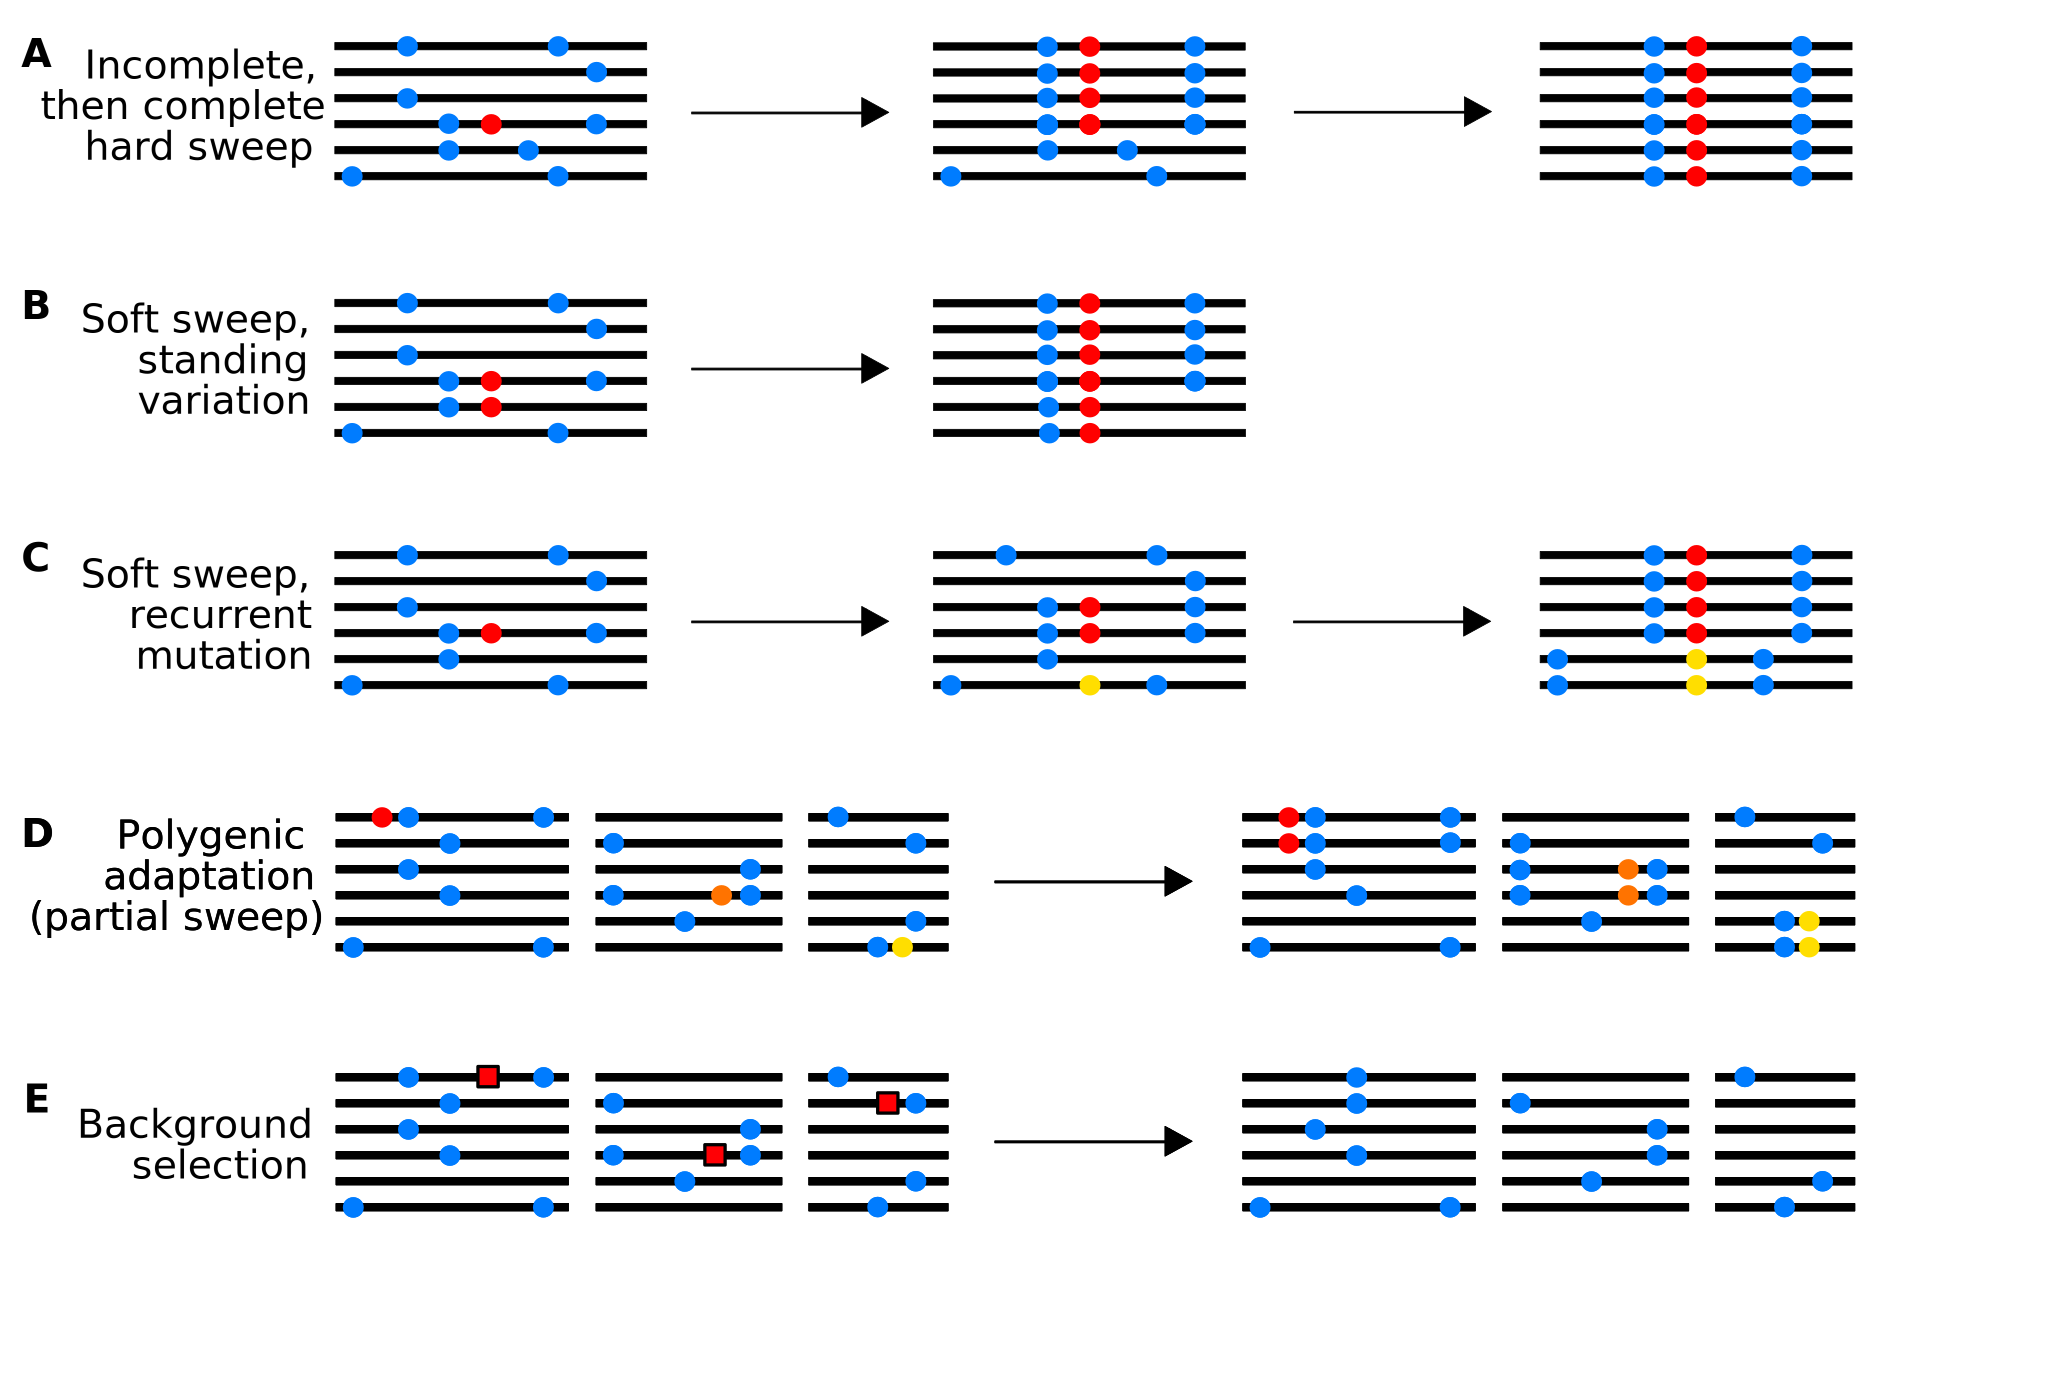
\includegraphics[width=\textwidth]{/Users/s0784966/Dropbox/Thesis/chapter1/figure_sweeps_no_legend.pdf}}
 \caption[Selective sweeps and background selection]{Selective sweeps and background selection. Blue circles are neutral varants, Reproduced from \cite{RN352}, thanks to Ben Jackson.}.
 
 \label{fig:sweepCartoon}
\end{figure}

\cite{RN124} showed that an advantageous mutation drags with it linked neutral polymorphisms as it rises in frequency. With increasing genetic distance from the selected site, the effect is reduced, resulting in troughs in genetic diversity in surrounding regions.
 
\emph{Hard/classic sweeps} \\
 
The most well-studied model of sweeps. A new advantageous mutation rapidly increases in frequency to eventual fixation (shown in Figure \ref{fig:sweepCartoon}-A). As it sweeps, the adaptive allele carries with it a portion of the haplotype on which it arose, reducing levels of neutral diversity in the surrounding area \citep{RN124,RN235}. \\
 
\emph{Soft sweeps} \\
  
A neutral allele segregating in a population may become favoured (due, for example, to a change in the environment). The segregating allele may be associated with multiple haplotypes, and as it rises in frequency, so do the multiple haplotypes (shown in \ref{fig:sweepCartoon}-B). A similar process, also termed a soft sweep, can occur if an advantageous mutation arises by multiple, distinct mutation events (shown in \ref{fig:sweepCartoon}-C). \\
 
\emph{Incomplete/partial sweeps} \\
 
If an advantageous allele increases in frequency, but does not reach fixation, there will still be some loss of linked neutral diversity. In this review we use the term incomplete sweeps to describe sweeps that are polymorphic at the time of sampling, but may (or may not) eventually reach fixation (shown in \ref{fig:sweepCartoon}-A). The term partial sweep describes the situation wherein a sweeping allele becomes effectively neutral at a certain frequency in its trajectory (shown in \ref{fig:sweepCartoon}-D). The magnitude of both processes on linked neutral diversity depend on the frequency reached by the sweeping allele when selection is ‘turned off’ or on the time of sampling \citep{RN226}. Partial sweeps may be common in cases of adaptation involving selection on quantitative traits \citep{RN147}. \\

\section[Using Models of Selective Sweeps to Estimate Positive Selection Parameters]{Using Models of Selective Sweeps to Estimate Positive Selection Parameters $^*$}
 
If adaptive substitutions are common, selection is expected to leave footprints in genetic diversity at linked sites. In particular, as a positively selected mutation increases in frequency, it tends to reduce diversity at linked neutral loci. Theoretical analysis of this process, termed a selective sweep, has shown that the reduction in diversity at a linked neutral locus depends on the ratio of the strength of positive selection to the recombination rate. Thus, comparing diversity at multiple neutral loci linked to selected regions, in principle, should provide an indirect means for estimating parameters of positive selection.
 

If a population experiences recurrent selective sweeps, there are several patterns predicted by theory. Under recurrent hard selective sweeps, levels of genetic diversity are expected to be lower i) in regions of the genome with restricted recombination, ii) in regions experiencing many sweeps and iii) in the genomic regions surrounding the targets of selection themselves. Each of these of these predictions have been met in empirical studies, and each has been used to estimate parameters of positive selection.


\subsection[The Correlation Between Diversity and the Rate of Recombination]{The Correlation Between Diversity and the Rate of Recombination $^*$}

In the late 1980s, evidence began to emerge suggesting that genetic polymorphism are less frequent in genomic regions experiencing restricted crossing-over \citep{RN225,RN282}. Soon after, \cite{RN114} showed that there is a positive correlation between nucleotide diversity and the rate of crossing-over in \emph{D. melanogaster}, a pattern subsequently observed in other eukaryotic species \citep{RN117}. Begun and Aquadro pointed out that the correlation is qualitatively consistent with the action of recurrent selective sweeps. \cite{RN277} formulated expressions, based on the correlation between nucleotide diversity and the rate of recombination, to estimate the compound parameter $\lambda 2N_{e}s$, where $\lambda$ is the rate of sweeps per base pair per generation, $N_e$ is the effective population size and $s$ is the selection coefficient. They applied their method to the data of \cite{RN114}, estimating $\lambda2N_{e}s$ = 5.37 x $10^{-8}$, but their method could not disentangle the individual parameters. More recently, \cite{RN226} performed a similar analysis in \emph{D. melanogaster} to explore the effects of partial sweeps on parameter estimates. They showed that when partial sweeps are common, the rate of adaptive evolution is underestimated if the hard sweep model is assumed.
 
The correlation between diversity recombination observed by \cite{RN114} can also be explained by background selection, the reduction in neutral diversity caused by the removal of linked deleterious mutations \citep{RN132}. The process of background selection is qualitatively similar to recurrent selective sweeps, since both processes reduce local genetic diversity \citep{RN110} and skew the SFS towards rare variants \citep{RN287,RN133}. Models of background selection envisage a neutral site linked to many functional sites at different distances, such that the effects of selection accumulate to reduce diversity \citep{RN206, RN157}. The correlation between neutral diversity and the recombination rate predicted by background selection is quantitatively similar to that observed in \emph{D. melanogaster} \citep{RN281}. Indeed, recent studies suggest that background selection is a major determinant of nucleotide diversity variation at broad scales ($>$100Kbp) in humans \cite{RN120} and \emph{D. melanogaster} \citep{RN288, RN116}. It is clear, then, that background selection is a key confounding factor when attempting to make inferences about positive selection.
 
\subsection[Correlations Between Neutral Diversity and Non-Neutral Divergence]{Correlation Between Neutral Diversity and Non-Neutral Divergence $^*$}

If there is a constant fraction of adaptive substitutions, $\alpha$, across the genome for a given class of sites, regions that evolve at higher rates should experience a greater number of selective sweeps. Under a model of recurrent sweeps, it follows that there should be a negative correlation between nucleotide divergence at selected sites and diversity at linked neutral sites. This was first described in \textit{Drosophila melanogaster} by \cite{RN283}, and has been subsequently reported in other \textit{Drosophila} species \citep{RN284}. Assuming a single rate of sweeps ($\lambda$) and a constant scaled strength of positive selection ($2N_es$) for a given class of sites, \cite{RN283} generalised formulae of \cite{RN277} based on the correlation between synonymous site diversity and non-synonymous site divergence to estimate  $\lambda 2N_es$ = $3 \times 10^{-8}$ for the X-chromosome in \textit{D. melanogaster}. Note that this $\lambda 2N_es$ estimate is similar to that obtained based on the correlation of synonymous site diversity and recombination rate (\cite*{RN277}; see above). Using an estimate of $\alpha = 0.50$ obtained from a MK-based analysis, \cite{RN283} decomposed the $\lambda 2N_es$ compound parameter, and inferred that $s \approx 0.001\%$ and $\lambda$ = $3.6 x 10^{-11}$ /bp/generation, suggesting that adaptation of protein-coding genes in \textit{D. melanogaster} is driven by moderately weak selection (i.e., assuming \textit{D. melanogaster} $N_e =10^6$, $2N_es \approx 40$). In a related study, Macpherson et al. (2007) estimated $\lambda 2N_es \approx 10^{-7}$ in \textit{D. simulans}, also by examining the correlation between mean neutral diversity and selected (nonsynonymous) divergence. However, their model also included the heterogeneity in levels of diversity, which is related to the rate and strength of sweeps in a different way to the mean, and allowed the individual parameters to be fitted by regression. The estimates of the compound parameter $\lambda 2N_es$ are similar between the two studies, though Macpherson et al. (2007) estimated that $s \approx 1\%$ (compared to Andolfatto’s estimate of $s \approx 0.001 \%$) and $\lambda = 3.6 \times 10^{-12}$ /bp/generation. The discrepancies between the studies may be due to differences in biology between the species, or may reflect methodological differences: For example, if the majority of adaptive substitutions are driven by weakly selected sweeps, which will leave a relatively small signal in levels of  polymorphism, the MK-based method may more sensitively detect them, perhaps explaining the higher rate of sweeps inferred by \cite{RN283}. On the other hand, strongly selected sweeps will leave a larger footprint in levels of diversity, so will be more readily detected using the approach of \cite{RN289}, perhaps explaining why they inferred a lower overall rate of sweeps, with higher selection coefficients (for a full description, see Sella et al. 2009). In both cases, inferences based on variation in polymorphism may reflect processes other than the fixation of adaptive alleles that have gone to fixation, such as partial sweeps and background selection, as these will affect patterns of diversity but not necessarily divergence. Related to this, the approach employed by \cite{RN283} has recently been extended by \cite{RN323}, by estimating the correlation between synonymous site diversity and non-synonymous divergence in the presence of both background selection and gene conversion in \textit{D. melanogaster}. They found that ignoring background selection tends to increase and decrease estimates of selection strength and rate, respectively. The parameter values estimated in their study suggest that 0.02\% of new mutations at nonsynonymous sites are strongly selected ($s \approx 0.03\%$, assuming $N_e$ = $10^6$ for \textit{D. melanogaster}).
 
\subsection[Patterns of Diversity Around the Targets of Selection]{Patterns of Diversity Around the Targets of Selection $^*$}
 
An individual hard selective sweep is expected to leave a trough in genetic diversity around the selected site. If a large proportion of amino acid substitutions are adaptive, as suggested by MK-type analyses (see above), collating patterns of diversity around all substitutions of a given type should reveal a trough in diversity. Such a pattern is not expected around a “control” class of sites, such as synonymous sites. This test, proposed by Sattath et al. (2011), was first applied it to \textit{D. simulans}, and the above pattern was found. By fitting a hard sweeps model to the shape of the diversity trough, they estimated α values of  5\% and 13\%, depending on whether one or two classes of beneficial mutational effects were fitted. Note that their estimates of α are substantially lower than those obtained using MK-based methods for \textit{D. melanogaster} (Andolfatto 2007). Sattath et al. (2012) suggested that modes of selection other than hard sweeps may help explain to this discrepancy. However, even when modelling two classes of beneficial mutations, they found that amino acid substitutions are driven by strongly adaptive mutations (s $sim0.5\%$ and s $\sim0.01\%$). Their estimates of selection strength are therefore in broad agreement with the estimate of s $sim1\%$ obtained by Macpherson et al. (2007), based on the correlation between synonymous diversity and non-synonymous divergence in \textit{D. simulans}. The Sattath et al. (2012) test, then, suggests that adaptation in protein-coding genes is fairly frequent and driven by strong, hard sweeps.
 
The Sattath test has been applied in a variety of organisms, including humans (Hernandez et al. 2011), wild mice (Halligan et al. 2013), \textit{Capsella grandiflora} (Williamson et al. 2014) and maize (Beissinger et al. 2016). In all but \textit{C. grandiflora}, researchers have found no difference in patterns of diversity around selected and neutral substitutions. These results have been interpreted as evidence that hard sweeps were rare in the recent history of both humans (Hernandez et al. 2011) and maize (Beissinger et al. 2016). However, Enard et al. (2014) pointed out that the Sattath test will be underpowered if there is large variation in levels of functional constraint in the genome. Indeed, through their analyses Enard et al. (2014) found evidence for frequent adaptive substitutions in humans, particularly in regulatory sequence. To address the issues raised by Enard et al. (2014), Beissinger et al. (2016) applied the Sattath test to substitutions in maize genes with the highest and lowest levels of functional constraint separately, but still found no difference in diversity pattern, suggesting either that hard sweeps have been rare in that species or that there is another confounding factor.
 
One possible explanation is that the species in which the Sattath test did/did not detect hard sweeps have distinct patterns of linkage disequilibrium (LD). LD decays to background levels within hundreds of base-pairs in \textit{D. simulans} \citep{RN283} and \textit{C. grandiflora} \citep{RN271}, whereas in humans, maize and wild mice it decays over distances closer to 10,000bp \citep{RN273,RN327, RN272}. It may be, then, that the Sattath test is only applicable when there is relatively short-range LD, such that the patterns of diversity around selected substitutions do not substantially overlap with the analysis windows around neutral ones. If this were the case, interpreting the similarity in troughs of diversity around selected and neutral substitutions as evidence for a paucity of hard selective sweeps may not be justified in organisms where LD decays over distances of a similar order of magnitude as the width of the diversity troughs themselves.
   	        	  
\section[Fitting genome wide patterns]{Fitting genome wide patterns $^*$}

	Methods to estimate the rate and strength of positive selection in the genome employ various combinations of nucleotide diversity, divergence, recombination rates and estimates of background selection effects as summary statistics, averaged over many regions of the genome. Recently, Elyashiv et al. (2016) developed a method that fits a model of hard sweeps and background selection to genome-wide variation in nucleotide diversity and divergence (at both selected and neutral sites). In \textit{D. melanogaster}, they showed that hard sweeps can explain a large amount of genome-wide variation genetic diversity. For nonsynonymous sites, they found that $\alpha = 4.1\%$ for strongly selected mutations ($s \geq 0.03\%$) and $\alpha = 36.3\%$ for weakly selected mutations ($s \approx 0.0003\%$), summing to $\alpha = 40.4\%$, which is similar to the estimate obtained using the MK-test \citep{RN283}. Their results suggest that accounting for weakly selected mutations may help reconcile the discrepancy between MK-based estimates of the rate and strength of selection and parameters estimated from sweep model predictions, described above.

\cite{RN274} showed that a map of the effects of hard sweeps and background selection is capable of explaining a large amount of the variation in diversity across the genome, further demonstrating that the action of natural selection is pervasive, at least in \textit{D. melanogaster}. However, their method overestimated the rate of deleterious mutations, which the authors attribute to the presence of modes of adaptation other than hard sweeps in \textit{D. melanogaster}. 


\section[Thesis aims]{Thesis aims}

	The aim of this thesis is further our understanding of the factors that shape variation in genetic diversity across the mammalian genome using the house mouse as a model. Particularly, I focus on the contributions of background selection and selective sweeps to variation in genetic diversity across the mouse genome. 

	The consequences of selection at linked sites are intrinsically linked to the rate of recombination. An understanding of how recombination rates vary across the genome is thus important for understanding how background selection and selective sweeps contribute to variation in genetic diversity across the genome.

	\begin{itemize}
	
	\item In Chapter 2, I leverage information from patterns of linkage disequilibrium across the mouse genome and construct recombination rate maps for the mouse genome. 
	
	\item In Chapter 3, I estimate the distribution of fitness effects both advantageous and deleterious mutations for multiple classes of sites in the mouse genome. I use these estimates to parametrise forward-in-time population genetic simulations. Using these simulations I ask, how 
	
	\item In Chapter 4, I fit a model incorporating the effects of both selective sweeps and background selection to troughs in diversity around functional elements in mice. Using the parameters that provide the best fit to the data, I ask whether adaptation in protein-coding or  regulatory regions contributes most to fitness in mice.
	
	\end{itemize}

